\documentclass[a4paper,10pt,hidelinks]{scrreprt}

% Packages =========================================
\usepackage{algorithm}
\usepackage{algpseudocode}
\usepackage{amsmath}
\usepackage{amsfonts}   		% Pakete für math. Formeln, Symbole, Ausdrücke
\usepackage{amssymb}
\usepackage[toc,page]{appendix}				% more control over appendices
\usepackage[english]{babel} 				% Anpassung für mehrsprachige Dokumente
\usepackage[utf8]{inputenc}				% for german characters like "ä, ö, ü"
\usepackage[safeinputenc=true,backend=biber,style=authoryear,natbib=true,maxbibnames=5,maxcitenames=1,uniquelist=false]{biblatex}
%\renewcommand*{\multinamedelim}{\semicolon\addspace}
\addbibresource{masterthesisbib.bib}
\usepackage[usenames, dvipsnames]{color}					% Nutzung von Farben
\usepackage{diagbox}
\usepackage{float}					% notw. für explizite Setzung von Grafiken
\usepackage[T1]{fontenc} 				% Zuweisung Codierschemas für Zeichensätze
\usepackage[paper=a4paper,left=40mm,right=30mm,top=20mm,bottom=25mm]{geometry} % Randmaße
\usepackage{graphicx} 					% Einbindung externer Grafiken
\usepackage{hyperref}
%\usepackage{listings}					% notwendig für Quellcode
\usepackage{lmodern}	 				% Moderne Version von Computer Modern
\usepackage{pdfpages}					% Einbindung einer pdf-Datei
\usepackage{pgfplots}
\usepackage{mdwlist}					% kompaktere Auflistungen
\usepackage{microtype}	 				% Optischer Randausgleich
\usepackage{subcaption}					% Subfigure/-tabellen
\usepackage{scrpage2}
\usepackage{tabularx}					% Textsetzung in Tabellen in p-Spalten
\usepackage{textcomp}					% Besondere Textzeichen
\usepackage{ulem}					% Unterstreichung
\usepackage{url}					% Links
\usepackage{xfrac}					% notw. für schräggestellten Bruch
\usepackage[margin=10pt,font=small,labelfont=bf,labelsep=endash]{caption}

% change this factor to change the spacing between rows in tables
\renewcommand{\arraystretch}{1.3}

% the following code avoids errors that come up if the abstracts in the .bib file contain %-signs
\DeclareSourcemap{ 
	\maps[datatype=bibtex]{
		\map{
			\step[fieldset=abstract, null]
		}
	}
}

\begin{document}
	\thispagestyle{empty}
	\begin{center}
		\Large
		\textbf{A Neuronal Model for Visually Evoked Startle Responses in Schooling Fish}\\
		
		\vspace*{1cm}
		\normalsize
		Master thesis\\
		
		\vspace{3cm}
		by\\
		Andrej Warkentin \\
		Bernstein Center for Computational Neuroscience - Berlin
		
		\vspace{2cm}
		Supervisors:\\
		Dr. Pawel Romanczuk\\
		Bernstein Center for Computational Neuroscience - Berlin\\
		Prof. Dr. Henning Sprekeler\\
		Technische Universit\"{a}t Berlin
		
	\end{center}
	\pagebreak 
	% Title Page
	\title{masterthesis}
	
	% Inhaltsverzeichnis =====================================
	\thispagestyle{empty}
	\tableofcontents		% Inhaltsverzeichnis erstellen
	\newpage
	%\cleardoublepage	% min. eine Freiseite
	
	%% Für den Hauptteil normale Seitenzahlen
	\pagestyle{useheadings}    % wieder auf normale Seitenrahmen zurück schalten
	\pagenumbering{arabic}  % Nummerierungstyp roman | arabic
	
	\begin{abstract}
		\textbf{Abstract}\\
		Many aspects of fish school behavior can be explained qualitatively by self-propelled agent models with social interaction forces that are based on either metric or topological neighborhoods.
		Recently, startling of fish has been analyzed in its dependence of the network structure 
		\citep{Rosenthal2015} but a mechanistic model and its influence on the collective behavior 
		is missing.
		Here we couple a model for collective behavior with a neuronal model that receives looming visual stimulus input to initiate a startle response, inspired by the neurobiologically well-studied Mauthner cell system.
		First, we analyzed the basic properties of the startle behavior of a single fish as a reaction to a looming stimulus.
		On the group level, we looked at startling frequency as well as group cohesion and polarization depending on neuronal and collective behavior parameters via simulations of the combined model.
		Our results indicate that the startling frequency strongly depends on the dynamics of the group structure, e.g. when the group approaches a boundary of the arena.
		In summary, we took first steps towards a biologically plausible model 
		for startle response initiation in the context of collective motion.
	\end{abstract}
	\newpage
	
	\chapter{Introduction}
	A common interpretation of the function of the nervous system in animals is to use the sensory 
	input in order to make appropriate actions.
	One situation where this would be useful for the animal is the sudden appearance of a predator.
	The quick response to such a sudden, unexpected stimulus is called startle response and can be 
	observed in many species \citep{Eaton1984a}.
	In fish, the startle response can take the form of freezing, where the fish	stops moving 
	entirely, or the form of an escape response, where it quickly accelerates and moves away within 
	less than a second.
	Escape responses in fish, also called fast starts, can be divided into the three stages 1) 
	first body bend, 2) second body bend and a third, variable stage where the fish either goes 
	into continuous swimming, coasting or braking \citep{Domenici2011}.
	Due to the body shape at the end of the first stage escape responses are also called C-start or 
	S-start \citep{Domenici2011}\footnote{It should be noted here that not all C-starts are escape 
	responses because they can also be involved in e.g. prey capture but we will ignore other roles 
	in the following.}.
	This thesis will focus on the C-start behavior of fish.\\
	The C-start behavior in fish has been extensively studied and one of the main reasons for this 
	is that a pair of neurons that play a major role in the initiation of the C-start, have large 
	soma and axons and are therefore relatively easy to find in experiments.
	They are called Mauthner cells (M-cells), named after Ludwig Mauthner who first found and 
	described their axons \citep{Mauthner1859}.\\
	Before going into the details of the M-cell circuit we will give a brief overview of the 
	nervous 
	system of fish to provide some context.
	Since we will later focus on visually evoked C-starts we will go into more detail when it comes 
	to the visual pathways in the brain.
	The overall structure of the nervous system of fish is very similar to mammals.
	Starting at the caudal end there is the spinal cord with descending motor pathways and the 
	ascending sensory pathways.
	The spinal cord goes over into the hindbrain region with the medulla and the cerebellum.
	This is followed by the midbrain which comprises the rostral part of the brainstem and a roof 
	region, the tectum \cite{the chapter in encyclopedia of fish physiology}.
	The remaining forebrain consists of the diencephalon and the telencephalon.
	%TODO: add appropriate references
	%TODO: say what is different in mammals/humans
	%TODO: mention somewhere that there are big differences among fish because there are so many 
	%species
	In terms of sensory organs fish are equipped with the same senses as mammals and additionally 
	have the lateral line organ that senses lower frequency signals around the body such as e.g. 
	water flow and in some cases organs that can sense electrical fields.\\
	%TODO: some transitional sentence to introduce the visual system
	Going from outside to inside, the eyes, again similar to mammals, consist of the cornea, the 
	lens surrounded by the iris and the retina followed by the photoreceptors which build the most 
	inside layer.
	In contrast to mammals the pupils of fish are not responsive to the amount of light in the 
	environment.
	Fish mostly have rods and three different cones although across species there are up to seven 
	different types of cones.
	The retina has different types of neurons that build different layers.
	The output neurons of the retina are the ganglion cells which show different kinds of tuning 
	and whose axons build the optic nerve when they exit the eye.
	%TODO: cite paper about tuning of retinal ganglion cells
	Although most fish don't have a fovea as we know it from humans there are retinal areas of 
	higher ganglion cell and photoreceptor densities \citep{Pita2015}.
	Most of the ganglion cell axons cross sides and end up in the optic tectum which is the 
	equivalent to the mammalian superior colliculus.
	While in humans much of the visual information goes further to the primary visual cortex in 
	fish the optic tectum is the main site of processing of visual information.
	Similar to cortical areas it is comprised of different layers, also receiving input from other 
	senses and other brain areas such as the telencephalon.
	The output of the optic tectum goes, among other regions, to the reticular nuclei in the 
	hindbrain where we also find the Mauthner cell and can thus come the M-cell circuit.\\
	The M-cell is located in the hindbrain and has two major dendritic branches, the ventral 
	dendrite and the lateral dendrite.
	It receives multisensory input which is divided between the two dendritic branches.
	The lateral dendrite receives auditory and lateral line input whereas the ventral dendrite 
	receives visual input via the optic tectum mentioned before.
	While this means that the visual input is highly processed by the networks in retina and optic 
	tectum before it arrives at the M-cell the auditory input comes directly from the auditory 
	nerve.
	This might be one of the reasons why the physiology of the auditory input has been studied in 
	more detail than the visual part.
	We will therefore continue to describe the properties of the auditory processing and will have 
	to assume that they also hold for the processing of the visual input.
	The synapses between auditory nerve and lateral dendrite are called club endings and transmit 
	auditory signals via electrical as well as chemical mechanisms which leads to Excitatory 
	Post-Synaptic Potentials (EPSPs) that consist of a fast and a slow component \citep{Korn2005}.
	At the same time the auditory nerve excites an interneuron which itself inhibits the M-cell.
	One interpretation of this feed-forward inhibition (FFI) is to increase the threshold for 
	initiating the startle response.
	But this is not the only function of these interneurons because they also inhibit the 
	contralateral M-cell as well as their contralateral counterparts \citep{Koyama2016}.\\
	This microcircuit is probably responsible for the decision of which direction to escape to.
	To illustrate why this connectivity makes sense in this decision-making context, let us 
	consider an auditory stimulus coming from the left side:
	It will inhibit the M-cell on the right side, inhibit the interneurons on the right side and 
	excite the M-cell on the left side.
	Effectively, we have an increased inhibition of the right M-cell, decreased inhibition of the 
	left M-cell and increased excitation of the left M-cell.
	Because the axons of the M-cells cross sides, an action potential of the M-cell on the left 
	side will lead to a contraction of muscles on the right side, resulting in movements of head 
	and tail away from the stimulus on the left side.\\
	There are further properties that seem to make the M-cell specialized for initiating the 
	C-start.
	Additional to the feed-forward inhibition the big size of the some of the M-cell leads to a 
	high input resistance which again increases the threshold for incoming currents to initiate an 
	action potential.
	The axon of the M-cell is unusually big as well which results in a fast signal transmission 
	when an action potential is initiated and thus allows for fast reactions.
	The axon is also connected to interneurons that provide feedback inhibition to both M-cells.
	This is thought to prevent repetitive firing of the M-cell that fired in the first place and 
	also to prevent the contralateral M-cell to fire shortly after.
	%TODO: check if axons are connected directly to interneurons
	%TODO: check what cranial relay neurons do and put it here
	Apart from this feedback inhibition the axon goes through the whole spinal chord with 
	colaterals that go to the motor neurons on the contralateral side.
	And also at this level we have again interneurons that putatively have the role of inhibiting a 
	different set of motor neurons that are responsible for steady swimming movements 
	\citep{Song2015}.\\
	The exact role of the M-cells and the surrounding circuit in the C-start behavior is still a 
	subject of study.
	The current state of research suggests that the M-cell is sufficient and necessary to evoke 
	the first phase of short-latency C-starts.
	%TODO: find reference and explain difference between short and long-latency c-starts
	Nevertheless, if the M-cell is ablated the fish are still able to perform long-latency C-starts 
	(\cite{Lacoste2015}, \cite{Dunn2016}).
	Furthermore, there is another population of neurons, that, if ablated, increase the latency of 
	C-starts in a similar manner as the ablation of the M-cell does \citep{Lacoste2015}.\\
	In the first part of this thesis we will make first steps towards a mechanistic understanding 
	of 
	functional role of the M-cell circuit for the C-start behavior.
	For this, we will greatly simplify the physiological properties of the M-cell and use a Leaky 
	Integrate-and-Fire (LIF) model to capture the relevant dynamics.
	We did not choose the more realistic Hodgkin-Huxley like model type that takes into account 
	different ion currents because we were not interested in the action potential shape but rather 
	in 
	the action potential timing dependent on the input.
	%TODO: maybe add reference to \cite{Brette2015}
	The simpler LIF model also allowed for more efficient simulation which was also useful for the 
	integration of the neuronal model in the collective behavior model in the second part.
	For the input of the M-cell we will assume that the visual input, coming from the optic tectum, 
	is the result of a feature extraction of the visual scene.
	Taken together, this will allow us to link parameters of the neuronal model to behavioral 
	response properties and to compare and fit this to experimental data.\\
	%TODO: mention looming stimulus experiments
	%TODO: describe previous work in "modeling the mauthner system"
	%TODO: mention rosenthal paper as motivation for the second part of the thesis
	While the first part of the thesis is concerned with the behavior of single fish, for many fish 
	species the natural environment is more likely to live in a group together with many other fish.
	Such groups of fish that move around together are called shoals if they are rather 
	uncoordinated and schools if they move in a highly ordered manner.
	This collective behavior is not well understood yet and in the second part of this thesis we 
	want to analyze how the startle response interacts with it.
	In more detail, we were interested in the following questions:
	Can the startle response be evoked spontaneously in the fish school e.g. when neighboring fish 
	come too close too fast?
	Does the startling of a single fish spread in the school?
	How do these effects depend on the properties of the school?\\
	In order to address these questions we will use an agent-based model that describes the 
	interactions between fish by so-called social forces.
	Typically, there are the three forces repulsion, alignment and attraction and they can work 
	either on neighbors within a specific range (metric interaction) or only on topological 
	neighbors (topological interaction).
	An example for a topological type of interaction would be to only consider the neighboring 
	cells of the Voronoi tessellation of the group of fish.
	Using such an agent-based collective behavior model with metric interaction, \cite{Couzin2002} 
	could show that the simulated fish school shows different modes of behavior dependent on the 
	parameters of the social forces.
	While in one mode the collective would be uncoordinated but stay loosely together, it would 
	move highly polarized and cohesive in another parameter regime or show a kind of milling 
	behavior in a third mode.
	%TODO: explain what we will do with this collective model
	%TODO: sum up and outline the remaining thesis
	\chapter{Single Mauthner Cell Model - Theory}
	In this chapter we will explain the theoretical aspects of the neuronal model for a single 
	Mauthner Cell.
	By 'single' Mauthner cell we only mean that we are considering the mechanisms of the 
	surrounding circuit involving one of the two existing Mauthner cells instead of both.
	We will start with the description of the full model and continue with two reductions that 
	assume a separation of timescales and thus provide stationary approximations of the model.
	\section{Full neuronal model}
	The full neuronal model of a single Mauthner cell consists of a rate-based model for the 
	population of inhibitory interneurons that provide the feed-forward inhibition and a LIF model 
	for the M-cell itself.
	Both the inhibitory population and the M-cell get their input from a single source.
	In our case this input will represent the visual information coming from the optic tectum which 
	will be described in more detail in the next chapter.
	The time evolution of the activity $\rho$ of the inhibitory population is described by the 
	following equation:
	\begin{equation}
	\tau _{\rho} \frac{d\rho}{dt} = - (\rho(t) - \rho_{0}) + c_{\rho} I(t) + 
	\eta _{\rho},
	\label{eq:inhib}
	\end{equation}
	where $\tau _{_\rho}$ is the time constant, $\rho _{0}$ is the resting activity of the 
	population, $c_{\rho}$ is a scaling factor, $I(t)$ is the time dependent input and $\eta 
	_{\rho}$ is a Gaussian noise term.
	For the M-cell we use a LIF model where the time evolution of the membrane potential $V_m$ is 
	described by the following equation:
	\begin{equation}
	\tau _m \frac{dV_m}{dt} = - (V(t) - E_{L}) + R_{m} I(t) - \rho (t) +  \eta 
	_m,
	\label{eq:mcell}
	\end{equation}
	where $\tau_{m}$ is the membrane time constant, $E_L$ is the resting potential, $R_m$ is the 
	membrane resistance and $\eta_{m}$ is again a Gaussian noise term.
	The M-cell thus gets the direct visual input $I(t)$ and is inhibited by $\rho(t)$.
	If the membrane potential $V_m$ crosses a threshold $V_t$ an action potential is artificially 
	produced and the membrane potential is reset to the resting potential $E_L$.
	Additional to the noise terms in equations \ref{eq:inhib} and \ref{eq:mcell} we will also 
	consider fluctuations of the firing threshold $V_t$:
	\begin{equation}
	V_t (t) = V_t + \eta_t,
	\label{eq:thrs}
	\end{equation}
	where $\eta_t$ is a Gaussian noise term.\\
	The basic parameters of the LIF model, i.e. $E_L$, $R_m$, $\tau_m$ and $V_t$, have been fitted 
	to experimental data in a previous study by \cite{Koyama2016} using recordings from four 
	%larval 
	zebrafish at four days post-fertilization(dpf).
	For the details of the fitting procedure see their methods section.\\
	One important property of this dynamic system are the time scales on which the described 
	activity is going on.
	Since we know that the synapses at the inhibitory interneurons are electric, at least for the 
	auditory input, the time constant, and therefore the relevant time scale, of $\rho$ is in the 
	order of milliseconds.
	As we will see later on, in the experiments that we want to reproduce the changes in the input 
	over time are on much bigger time scales of at least hundreds of milliseconds.
	This fact motivates the reduction in the next section where we approximate the activity of the 
	inhibitory population by the stationary solution.
	\section{Stationary Approximation of Inhibitory Population}
	Here we reduce the model by approximating the activity of the inhibitory population by its 
	stationary solution.
	This approximation is the more accurate the higher the difference is between the time scale of 
	the dynamics of the inhibitory population and the time scale of the input.
	If we use $\tau_{\rho}$ as the time scale of the inhibitory population and denote $\tau_{in}$ 
	as the time scale of the input, the approximation becomes equivalent for the limit 
	$\tau_{\rho}/ \tau_{in} \rightarrow 0$.
	In the model, this means that equation \ref{eq:inhib} becomes:
	\begin{equation}
	\hat{\rho} (t) = \rho_{0} + c_{\rho} I(t) + \eta_{\rho}.
	\label{eq:inhib_approx}
	\end{equation}
	Now we can replace $\rho (t)$ in equation \ref{eq:mcell} and get:
	\begin{equation}
	\tau _m \frac{dV_m}{dt} = - (V(t) - E_{L}) + I(t)(R_{m} - c_{\rho}) - \rho_{0} - 
	\eta_{\rho} +  \eta _m.
	\label{eq:mcell_approx1}
	\end{equation}
	In the resulting LIF model the input is now weighted by the difference between the scaling 
	factor $c_{\rho}$ and the membrane resistance $R_m$.
	If we ignore the noise terms for a moment and assume that $\rho_{0}=0$, this means that the 
	input can only excite the M-cell and therefore evoke an action potential if $c_{\rho} < R_m$.
	Increasing $\rho_{0}$ would effectively increase the firing threshold $V_t$.
	\section{Stationary Approximation of Full Model}
	As a next step we can further approximate the LIF model in equation \ref{eq:mcell_approx1} by 
	its stationary solution:
	\begin{equation}
	\hat{V}_m(t) = E_{L} + I(t)(R_{m} - c_{\rho}) - \rho_{0} - 
	\eta_{\rho} +  \eta _m.
	\end{equation}
	If we set all noise to zero we can derive an expression for the input at which the membrane 
	potential reaches the threshold $V_{t}$:
	\begin{equation}
	\hat{V}_m(t) \overset{!}{=} V_t
	\end{equation}
	\begin{equation}
	\Leftrightarrow E_{L} + I(t)(R_{m} - c_{\rho}) - \rho_{0} 
	\overset{!}{=} V_t
	\end{equation}
	\begin{equation}
	\Leftrightarrow I(t)
	\overset{!}{=} \frac{V_t - E_{L} + \rho_{0}}{(R_{m} - c_{\rho})}
	\label{eq:crit_input}
	%TODO: look up solution for simple LIF equation even if it's only for linear input
	%TODO: say that this is comparable to first-passage time problems such as in the 
	%drift-diffusion model for decision making(maybe cite ratcliff2002 or so)
	\end{equation}
	\begin{itemize}
		\item maybe discuss relation to first-passage time problems
	\end{itemize}


	\chapter{Single Mauthner Cell Model - Numerical experiments}
	We will now come to the simulations of the visual looming stimulus experiment.
	For this we first describe the experiments that we want to reproduce, especially the specific 
	conditions and results.
	This is followed by the results of the simulations using the model in the different 
	formulations that we showed in the previous chapter.
	Furthermore, we fit the parameters of the full model to experimental data and finally summarize 
	and discuss our findings.
	\section{Visual looming stimulus experiments}
	One of the earliest visual looming stimulus experiments has been conducted by 
	\cite{Dill1974} where they photographed a black dot on a white background and projected these 
	photographs on a tracing paper that was taped to the wall of the aquarium and thus creating a virtual looming stimulus.
	They also tested a model predator that consisted of a black disk of Plexiglas that was moved by a motor.
	In more recent studies computer-generated stimuli are used and therefore the stimulus size 
	and velocity can be controlled more precisely.\\
	The typical arrangement is a small dish or aquarium in which a single fish can either freely 
	move or it is head-restrained, i.e. it can only move its tail while the head is fixed. 
	In the studies that we will consider here they used larval zebrafish (\cite{Temizer2015}, 
	\cite{Dunn2016}, \cite{Bhattacharyya2017}) and in one case they used goldfish 
	\citep{Preuss2006}.
	The stimulus is then either projected on the floor, ceiling or side wall of the aquarium or a 
	screen is placed close to the aquarium.
	In most studies the stimulus is a black disk or square on a white or blue background.
	Other stimuli that have been tested, such as a circle with a checkerboard pattern did not show significant differences (\cite{Preuss2006}, \cite{Dunn2016}) but there has been no systematic analysis .
	The stimulus sizes, i.e. the diameter of the disk or the side length of the square, range from 0.3 mm to 5 cm and the velocities range from 0.2 cm/s to 60 cm/s.
    Another parameter that is often reported is the ratio of stimulus size and velocity, L/V, which indicates the time needed to cover a distance of a length equal to the stimulus size.
	The subtended visual angles on the retina of the fish range from 2\textdegree to at least 
	100\textdegree.
	For an overview of all reported conditions in the experiments see Table \ref{tab:looming_exp}.\\
	\begin{table} [!th]
		\begin{center}
			\begin{tabular}{l|c|c|c|c}
				%\hline
				\textbf{Study} & \textbf{1} & \textbf{2} & \textbf{3} & \textbf{4}\\
				\hline
				\textbf{Species} & Zebrafish & Zebrafish & Zebrafish & Goldfish\\
				%\hline
				\textbf{Age} & 6-8 dpf & 5-6 dpf & 5 - 7 dpf & -\\
				%\hline
				\textbf{Water temperature [\textdegree C]} & 28  & - & 24  & 18 \\
				%\hline
				\textbf{Screen spanning} & 62 & >100* & >70* & -\\
				\textbf{angle horizontal [\textdegree]} & & & & \\
				%\hline
				\textbf{Screen spanning} & 50 & - & - & -\\
				\textbf{angle vertical [\textdegree]} & & & & \\
				%\hline
				\textbf{Screen distance [cm]} & 1 & - & 3.25 & 16\\
				%\hline
				\textbf{Luminance dark} & 0.07 cd/$m^2$ & 0.7 lux & - & 70-80 lux\\
				%\hline
				\textbf{Luminance grey} & - & 75 lux & - & -\\
				%\hline
				\textbf{Luminance white} & 122.5 cd/$m^2$ & 512 lux & 500 lumen & 300-320 lux\\
				%\hline
				\textbf{L/V values [ms]} & 60-300 \dag & 510 - 2900 \dag & 100 - 
				1200 & 20 - 110*\\
				%\hline
				\textbf{Durations [s]} & 1.65 - 8 & 0.5 - 5* & 1 - 5.5* & 0.25 - 0.8*\\
				%\hline
				\textbf{Acclimation time [min]} & - & - & 15 & -\\
				%\hline
				\textbf{Visual angles [\textdegree]} & 2 - 48 & 25 - 100* & 8 - 70* & 2 - 100*\\
				%\hline
				\textbf{Critical angle [\textdegree]} & 21.7 $\pm$ 2.5 & 72 $\pm$ 1.3 & 35 $\pm$ 15 
				& -\\
				%\hline
				\textbf{Response probabilities} & 20 - 75* & 46 - 60 & 25 - 75* & 70 - 91\\
				%\hline
				\textbf{Head-restrained} & Yes & No & No & No\\
				%\hline
				\textbf{Stimulus shape} & Circle & Circle & Rectangle & Circle\\
				%\hline
				\textbf{Stimulus color} & Black/White, & Black/Chkb. & Black & Black\\
				%\hline
				\textbf{Background color} & White/Black, & Grey & Blue & White\\
				%\hline
				\textbf{Stimulus sizes [cm]} & 0.03 & ? & 1 - 2.5 & 0.5 - 5*\\
				%\hline
				\textbf{Stimulus velocities [cm/s]} & 0.2 - 1 & ? & ? & 20 - 60\\
				%\hline
				\textbf{Initial distances} & ? & ? & 5 & ?\\
				\textbf{(virtual) [cm]} &  &  &  & \\
				%\hline
				\textbf{Projection site} & Side/Front & Bottom & Side/Front & Above\\
				%\hline
			\end{tabular}
		\end{center}
		\caption{The corresponding references of the studies are 1: \cite{Temizer2015}, 
		2: \cite{Dunn2016}, 3: \cite{Bhattacharyya2017} and 4: \cite{Preuss2006}.
		Note that the studies might have conducted other looming stimulus experiments with 
		simultaneous neural recordings but they are not included here because this project is 
		restricted to the behavioral aspects.
		For values denoted with a "\dag" we used the diameter 
		instead of the radius, as it was done in the original studies.
		Values with an "*" are either 
		read of figures or inferred from other, reported values. Chkb. = Checkerboard pattern.}
		\label{tab:looming_exp}
	\end{table}
	%TODO: make appropriate groups for table and/or remove some of them and put the full table into 
	%appendix
	For the results of the experiment the time from onset of the stimulus (latency), the distance and the 
	visual angle are measured at the time when the fish responds, i.e. starts to move away.
	The visual angle at response time (response angle) has been found to have the same mean value 
	at different stimulus sizes and velocities in all studies that were done with zebrafish, 
	although there are substantial differences in the mean value as well as in the variance.
	This could be explained by the differences in various experimental conditions such as the water 
	temperature, head restraining or the acclimation time (see Table \ref{tab:looming_exp}).
	While the study with goldfish \citep{Preuss2006} does not report to find a so-called critical visual angle, the observed response angles (14\textdegree to 29\textdegree) are in a range 
	that is comparable to e.g. the one found by \cite{Bhattacharyya2017} (35\textdegree $\pm$ 
	15\textdegree).\\
	For the simulations of the experiment we closely followed the procedure reported by 
	\cite{Bhattacharyya2017}.
	At the beginning of a trial a stimulus size is drawn from a uniform distribution between 10 mm and 25 mm.
	Next, an L/V value is uniformly drawn between 0.1 s and 1.2 s and the resulting velocity for the 
	trial stimulus size is calculated.
	With the trial stimulus size $L_{trial}$ and the trial velocity $v_{trial}$ the visual angle 
	over time $\theta(t)$ is calculated by:
	\begin{equation}
	\theta (t) = 2\cdot \arctan(\frac{L_{trial}/2}{D_{init} - v_{trial}\cdot t}),
	\label{eq:theta}
	\end{equation}
	where $D_{init}$ is the virtual initial distance which is set to 50mm if not stated otherwise.
    The range of possible time courses of the visual angle is shown in Figure \ref{fig:theta_lv} A.
    Note that because the initial distance is fixed and we sample from different stimulus sizes we get different initial angles for the same L/V values.
    This leads to different time courses for the same L/V value depending on the stimulus size but starting from the same angle their time courses are identical (Figure \ref{fig:theta_lv} B).
    If we now assume a critical angle $\theta_{crt}$ at which the fish escapes, we can describe how the response time, response distance and time-to-collision (TTC) at response depend on the L/V value.
    The response time linearly depends on the L/V while the slope of the relationship is determined by stimulus size $L$, initial distance $D_{init}$ and critical angle $\theta_{crt}$:
	\begin{equation}
	t_{resp} = \dfrac{L}{v} \left(\dfrac{D_{init}}{L} - \dfrac{1}{2\cdot\tan(\theta_{crt} /2)}\right).
	\label{eq:resp_time}
	\end{equation}
    The response distance only depends on the stimulus size $L$:
    \begin{equation}
	D_{resp} = \dfrac{L}{2\cdot \tan(\theta_{crt} /2)}.
	\label{eq:resp_dist}
	\end{equation}
    The TTC linearly depends on $L/V$ and the slope is determined only by the critical angle $\theta_{crt}$:
	\begin{equation}
	TTC_{resp} = - \dfrac{L}{2\cdot v\cdot \tan(\theta_{crt} /2)}.
	\label{eq:resp_ttc}
	\end{equation}
    For an example with $\theta_{crt}=35$ and $D_{init}=50$ these idealized response properties are illustrated in Figure \ref{fig:ideal_resp_props}, where we chose the same axes as in Figure 1 of \cite{Bhattacharyya2017} for easy comparison.\\
	In our simulations the visual angle is next transformed by a linear function and the result is the input $I(t)$ for our neuronal model, described in the previous chapter:
	\begin{equation}
	I(t) = f(\theta (t)) = m \cdot \theta(t) + b.
	\label{eq:input}
	\end{equation}
	In order to calculate the response properties we take the time of the first spike $t_{spk}$ of the model M-cell after stimulus onset as the response time of the fish.
	We ignore further processing time after the spike because it is in the order of milliseconds \citep{Preuss2003} and thus irrelevant with respect to the overall response time which is in the order of at least hundreds of milliseconds for visual stimuli \citep{Preuss2006}.
	Thus the response angle of the simulated trial will be $\theta (t_{spk})$.
	%TODO: mention initial period with constant size
	
    \begin{figure}[!h]
    	\begin{center}
			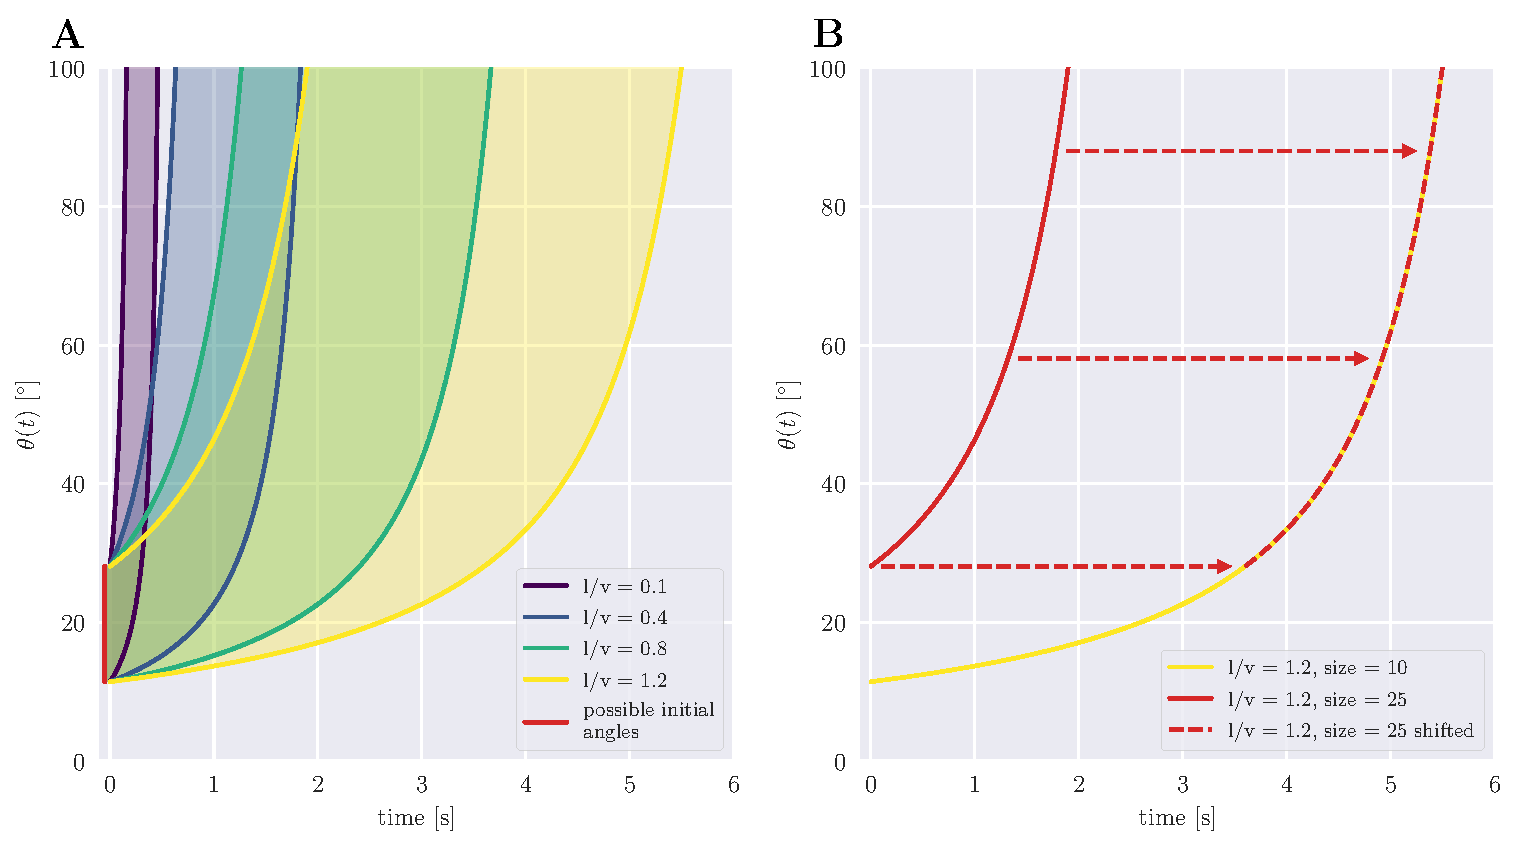
\includegraphics[width=\textwidth]{figure_theta_lv_test.pdf}
    	\end{center}
    	\caption{Range of time courses of $\theta$ depending on L/V. \textbf{A} For four different L/V values the possible time courses are shown if stimulus size L ranges between 10 mm and 25 mm. \textbf{B} Single time courses for the same L/V value only differ in a horizontal shift that is introduced by the different initial angle.}
    	\label{fig:theta_lv}
    \end{figure}
    
    \begin{figure}[!h]
    	\begin{center}
			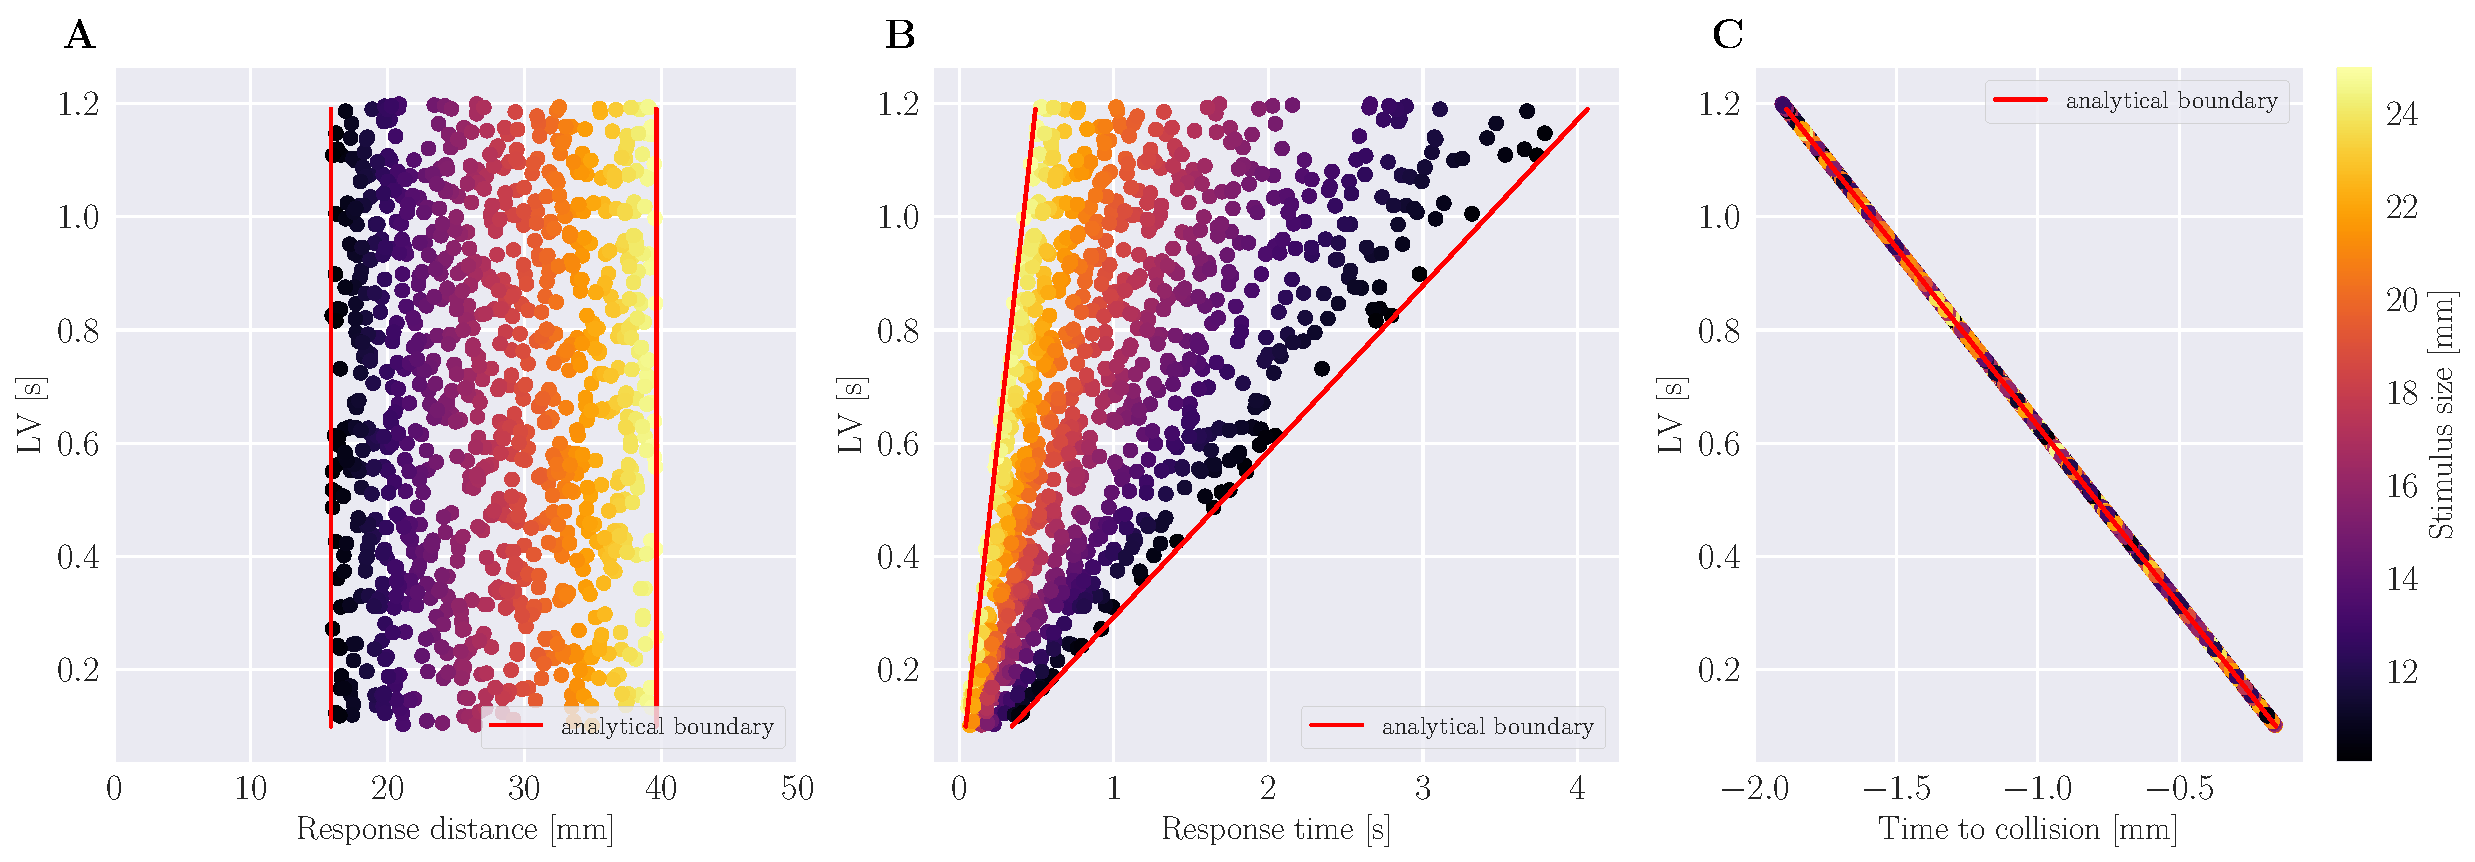
\includegraphics[width=\textwidth]{figure_ideal_resp.pdf}
    	\end{center}
    	\caption{Response properties for a critical angle $\theta_{crt}=35$ and initial distance $D_{init}=50 mm$.  For all plots L was sampled between 10 mm and 25 mm and L/V was sampled between 0.1 s and 1.2 s. Red lines show minimal and maximal values calculated using Equations \ref{eq:resp_time}, \ref{eq:resp_dist} and \ref{eq:resp_ttc}. \textbf{A} The response distance only depends on L and thus has the same range for all L/V values. \textbf{B} Response times linearly increase with L/V and the slope increases for smaller L. \textbf{C} Absolute time-to-collision linearly increases with L/V and the slope only depends on $\theta_{crt}$.}
    	\label{fig:ideal_resp_props}
    \end{figure}
		
	\section{Stationary model prediction}
	\begin{equation}
	I(t) = 10^{-11} c_{exc} f(\theta(t)) = 10^{-11} c_{exc} (m \cdot \theta(t) 
	+ b)
	\end{equation}
	Inserting values for the fixed parameters $E_{L}=-79$ mV, $R_{m}=10$ 
	M$\Omega$ 
	and $V_{t}=-61$ mV:
	\begin{equation}
	-0.079 + 10^{7} I(t) - c_{\rho} 10^{7} I(t) - \rho_{0} \overset{!}{=} -0.061
	\end{equation}
	
	\begin{equation}
	\Leftrightarrow 10^{7} I(t) - c_{\rho} 10^{7} I(t) - \rho_{0} 
	\overset{!}{=} 0.018
	\end{equation}
	
	\begin{equation}
	\Leftrightarrow 10^{-4} c_{exc} f(\theta(t)) (1 - c_{\rho}) - \rho_{0} 
	\overset{!}{=} 0.018
	\end{equation}
	
	\begin{equation}
	\Leftrightarrow f(\theta(t)) \overset{!}{=} \frac{180 + \rho_{0}10^{4}} 
	{c_{exc}(1 - c_{\rho})}
	\end{equation}
	
	\begin{equation}
	\Leftrightarrow \theta(t) \overset{!}{=} \frac{180 + \rho_{0}10^{4}} 
	{m \cdot c_{exc}(1 - c_{\rho})} - \frac{b}{m}
	\end{equation}
	\section{Chapter outline}
	\begin{itemize}
		\item results for the minimal model aka the noiseless, stationary solution:
		\begin{itemize}
			\item we know expression for critical input from equation \ref{eq:crit_input}
			\item if we insert our expression for the visual looming stimulus we get this critical 
			angle as a function of the free parameters: show equation
			\item optional: what happens if we use sigmoid function instead of linear?
		\end{itemize}
		\item results for simple LIF model where inhibitory population activity is approximated:
		\begin{itemize}
			\item show response properties (only 2 or 3 as the others are redundant) and their 
			dependence on free parameters: 
			\item also always include stationary solution from previous section for comparison
			\item also show preuss data
		\end{itemize}
		\item results for full model:
		\begin{itemize}
			\item show effect of additional parameter $\tau_{\rho}$
		\end{itemize}
		\item fitting of parameters:
		\begin{itemize}
			\item we will only use raw data that we got from \cite{Bhattacharyya2017} bc it's from 
			zebrafish where we have the fitted parameters from \cite{Koyama2016}
			\item give brief summary of fitting procedure from \cite{Lueckmann2018}
			\item describe chosen meta parameters for fitting: layers, neurons per layer, nepochs, 
			ntraining runs etc.
			\item show fitting results
		\end{itemize}
		\item discussion of results:
		\begin{itemize}
			\item summarize results
			\item mention stimulus time scales
			\item unifying theory that combines bhattacharyya data and preuss data?!
			\item do fitted parameters make sense?
		\end{itemize}
	\end{itemize}
	\begin{table} [!th]
		\begin{center}
			\begin{tabular}{l|c|p{7cm}}
				%\hline
				\textbf{Parameter} & \textbf{Value (unit)} & \textbf{Comment} \\
				\hline
				$E_L$ & -79 mV & Resting potential\\
				$R_M$ & 10 MOhm & Membrane resistance\\
				$\tau_{m}$ & 23 ms & Membrane time constant\\
				$V_t$ & -61 mV & Mean spiking threshold\\
				$dt$ & 0.001 s & Integration time step\\
				$T$ & 5 s & Total time\\
				$sd_{thr}$ & 1 mV & Standard deviation of spiking threshold noise\\
				$sd_{I}$ & 5 mV & Standard deviation of input noise\\
				$sd_{init}$ & 1 mV & Standard deviation of initial condition noise\\
				$m$ & 1 \textdegree/s  & Slope of linear transformation\\
				$b$ & 0 \textdegree & Offset of linear transformation\\
				%\hline
			\end{tabular}
		\end{center}
		\caption{Parameters of the single LIF neuron model with a looming stimulus input. Parameters that were explored are indicated either by a value range such as e.g. for $\mu_s$ or by a set with all explored values inside of curly brackets such as e.g. for $\sigma_s$.}
		\label{tab:neuroparams}
	\end{table}
	%\chapter{Two Mauthner Cells Model}
	\chapter{Coupling of Neuronal Model and Collective Dynamics}
	\begin{itemize}
		\item description behavioral experiments:
		\begin{itemize}
			\item schooling behavior in general has been analyzed
			\item startling in schools has not been studied so much (except maybe 
			\cite{Fischer2015})
			\item but there is study by \cite{Rosenthal2015}
			\item summarize experiment and findings
		\end{itemize}
		\item description schooling model:
		\begin{itemize}
			\item movement equations, social forces (take from lab report)
			\item describe coupling: every agent integrates visual info (how will be described in 
			next section)
			\item decision: on what level should we implement the variability of rho null? over 
			time or across fish? we chose across fish here, assuming they are in different internal 
			states, maybe also with different characters (cite paper about dominance 
			\cite{Khan2017}, \cite{Miller2017}, \cite{Neumeister2010}, \cite{Park2018})
		\end{itemize}
		\item how to integrate visual info/couple input from different neighbors
		\begin{itemize}
			\item mention ensemble statistics (see paper that pawel sent me)
			\item what we will look at: global mean/max/deviate, knn mean/deviate
		\end{itemize}
		\item simulation results:
		\begin{itemize}
			\item show startle frequency, density and polarization for the different integration 
			strategies
			\item show effect of school position on startle probability
			\item show cascade sizes as function 1)input scaling 2) school structure, order, density
			
		\end{itemize}
	\end{itemize}
	\chapter{Discussion}
	\begin{itemize}
		\item we focus here on the experimental results from 
		\cite{Bhattacharyya2017} but one should keep in mind that their results 
		might be specific to properties of experiment such as fish handling, 
		fish age, species, arena, environment, stimulus setup (projection on 
		screen)
		\item we took the fitted parameters from \cite{Koyama2016} but those are fitted for their 
		specific context which might vary in other experimental conditions and certainly in other 
		species
		\item furthermore the LIF model makes strong assumptions about the processing power of the 
		neuron which are likely not true. see for example \cite{Koch2000}, and specifically for 
		%the 
		M-cell \cite{Medan2017}
		\item in locusts, neurons have been found that specifically code looming stimuli 
		\cite{Hatsopoulos1995} (?)
		\item we should keep in mind that the optic tectum is still developing at larval stage 
		\cite{Avitan2017}
		\item considering the amount of differences of previous studies that looked into visual 
		looming stimuli, a more systematic analysis of visually evoked startle responses in 
		zebrafish is clearly missing
		\item test citations: \cite{Severi2014}, \cite{Sarvestani2013}, \cite{Romano2015}, 
		\cite{Parrish2002}, \cite{Moeller1989}, \cite{Howe2013}, \cite{DelBene2010}
	\end{itemize}
	\newpage
	%\bibliographystyle{abbrvnat}
	%\bibliography{masterthesisbib}
	\printbibliography[heading=bibintoc]
	
	\newpage
	\appendix
	%\appendixheaderon
		% next line tells latex to not list sections in the Table of Contents, \protect is needed because \setcounter apparantly
		% is a fragile command (see http://www.tex.ac.uk/FAQ-protect.html)
	\addtocontents{toc}{\protect\setcounter{tocdepth}{-1}}
	\section{Appendix}

	
\end{document}          
